\documentclass{article}

\usepackage[utf8]{inputenc}
\usepackage[letterpaper, total={6in, 9in}]{geometry}
\usepackage{amsmath}
\usepackage{natbib}
\usepackage{wrapfig}
\usepackage{graphicx}
\usepackage{amssymb}
\usepackage{tikz}
\usepackage{array}

\title{Combinatorics}
\author{TSS Math Club}
\date{March 2023}

\begin{document}
\large

\maketitle

\section{Introduction to Counting}

\subsection{Rule of Product}

\subsubsection{Definition}
\vspace{20px}
\subsubsection{Tree Diagram}
\vspace{80px}
\subsubsection{Example 1}
How many 4 digit numbers are there with no repeated digits?
\vspace{20px}

\subsubsection{Example 2}
How many 5 digit odd numbers are there with no repeated digits?
\vspace{20px}

\subsubsection{Example 3}
How many ways are there for 5 people to stand in a row?
\vspace{20px}



\subsection{Rule of Sum}

\subsubsection{Definition}

\vspace{20px}
\pagebreak
\subsubsection{Example 1}
Calvin wants to go to Milwaukee. He can choose from 3 3 bus services or 2 2
train services to head from home to downtown Chicago. From there, he can choose
from 2 bus services or 3 train services to head to Milwaukee. How many ways are
there for Calvin to get to Milwaukee?
\vspace{30px}



\subsection{Case Working}
\subsubsection{Definition}
\vspace{20px}
\subsubsection{Example 1}
How many numbers less than 10,000 are there with no repeated digits?
\vspace{20px}

\subsubsection{Example 2}
Consider the flag:


\tikzset{every picture/.style={line width=0.75pt}} %set default line width to 0.75pt        

\begin{tikzpicture}[x=0.75pt,y=0.75pt,yscale=-1,xscale=1]
%uncomment if require: \path (0,585); %set diagram left start at 0, and has height of 585

%Shape: Rectangle [id:dp9161151772239684] 
\draw   (100,112) -- (226.48,112) -- (226.48,196.03) -- (100,196.03) -- cycle ;
%Shape: Rectangle [id:dp21041871757069686] 
\draw   (226.48,112) -- (352.96,112) -- (352.96,196.03) -- (226.48,196.03) -- cycle ;
%Shape: Rectangle [id:dp24653680549059187] 
\draw   (100,196.13) -- (226.48,196.13) -- (226.48,280.16) -- (100,280.16) -- cycle ;
%Shape: Rectangle [id:dp08301293915445807] 
\draw   (226.48,196.13) -- (352.96,196.13) -- (352.96,280.16) -- (226.48,280.16) -- cycle ;




\end{tikzpicture}\\
If 10 colours are provided, how many ways are there to colour the flag so that no 2 adjacent regions have the same colour.
\vspace{20px}

\subsection{Indirect/Complementary Counting}
\subsubsection{Example 1}
How many positive integers less than $100$ are not a multiple of five?
\vspace{20px}

\subsubsection{Example 2}
How many four-digit positive integers have at least one digit that is a 2 or a 3?
\pagebreak

\subsection{Venn Diagram and Inclusion-Exclusion Principle}

\subsubsection{Venn Diagram}

Example:
100 students were interviewed.
28 took PE, 31 took BIO, 42 took ENG, 9 took PE and BIO, 10 took PE and ENG, 6 took BIO and ENG, 4 took all three subjects.
\begin{itemize}
    \item How many students took none of the three subjects?
    \item How many students took PE but not BIO or ENG?
    \item How many students took BIO and PE but not ENG?
\end{itemize}
\tikzset{every picture/.style={line width=0.75pt}} %set default line width to 0.75pt        

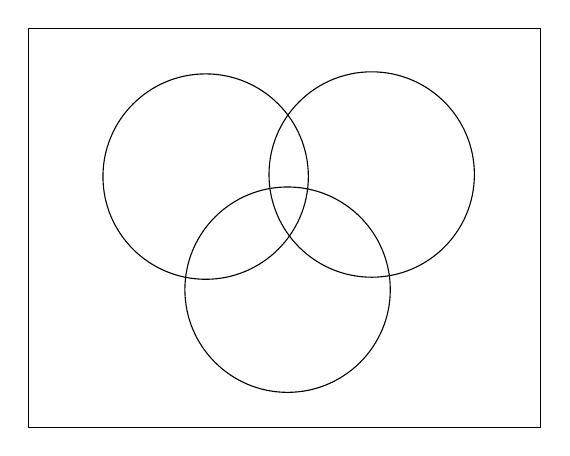
\begin{tikzpicture}[x=0.75pt,y=0.75pt,yscale=-1,xscale=1]
%uncomment if require: \path (0,585); %set diagram left start at 0, and has height of 585

%Shape: Rectangle [id:dp8186228115590011] 
\draw   (63,71) -- (309.96,71) -- (309.96,263.16) -- (63,263.16) -- cycle ;
%Shape: Circle [id:dp002176999662527823] 
\draw   (99,142.48) .. controls (99,115.15) and (121.15,93) .. (148.48,93) .. controls (175.81,93) and (197.96,115.15) .. (197.96,142.48) .. controls (197.96,169.81) and (175.81,191.96) .. (148.48,191.96) .. controls (121.15,191.96) and (99,169.81) .. (99,142.48) -- cycle ;
%Shape: Circle [id:dp6218005090315404] 
\draw   (138.48,196.96) .. controls (138.48,169.63) and (160.63,147.48) .. (187.96,147.48) .. controls (215.28,147.48) and (237.44,169.63) .. (237.44,196.96) .. controls (237.44,224.28) and (215.28,246.44) .. (187.96,246.44) .. controls (160.63,246.44) and (138.48,224.28) .. (138.48,196.96) -- cycle ;
%Shape: Circle [id:dp7933760637768881] 
\draw   (179,141.48) .. controls (179,114.15) and (201.15,92) .. (228.48,92) .. controls (255.81,92) and (277.96,114.15) .. (277.96,141.48) .. controls (277.96,168.81) and (255.81,190.96) .. (228.48,190.96) .. controls (201.15,190.96) and (179,168.81) .. (179,141.48) -- cycle ;




\end{tikzpicture}
\vspace{20px}

\subsubsection{Inclusion-Exclusion Principle}
Two sets: $|A_1 \cup A_2| = |A_1| + |A_2| - |A_1\cap A_2|$.\\
Three sets: $|A_1\cup A_2\cup A_3| = |A_1| + |A_2| + |A_3| -|A_1\cap A_2| - |A_2\cap A_3| - |A_3\cap A_1| +|A_1\cap A_2\cap A_3|$.\\
\\
Example:\\
There are $20$ students participating in an after-school program offering classes in yoga, bridge, and painting. Each student must take at least one of these three classes, but may take two or all three. There are $10$ students taking yoga, $13$ taking bridge, and $9$ taking painting. There are $9$ students taking at least two classes. How many students are taking all three classes?
\pagebreak

\section{Permutation and Combination}

\subsection{Factorial}
\subsubsection{Notation/Definition}
$n!=$
\subsubsection{Examples}
\begin{itemize}
    \item $3!=$
    \item $5!=$
    \item $(n^2+5n+6)(n+1)!=$ 
\end{itemize}

\subsection{Permutation}
\subsubsection{Definition}
\vspace{20px}
\subsubsection{Notation}
$mPn=P(m,n)=$
\subsubsection{Examples}
\begin{itemize}
    \item $5P3=$
    \item $P(7,2)=$
    \item $P(n,r)P(n-r,m)=$ 
\end{itemize}
\subsection{With Repetition}
\subsubsection{No repetiotion}
How many arrangements are there for the word MATHS?
\vspace{20px}
\subsubsection{With repetiotion}
How many arrangements are there for the word TORONTO?
\vspace{20px}
\subsubsection{Problem}
How many ways can 12 basketball players be assigned to four triple rooms?
\pagebreak

\subsection{Grouping}
\subsubsection{Example}
Math Club is taking yearbook photo one day with 20 members and Mr.Fraschetti and Mr.Gatti lining in a row. If Mr.Fraschetti and Mr.Gatti insist to stand together, how many arrangements are there?
\vspace{20px}
\subsubsection{Problem}
At a recent conference of the 11 premiers (including the Prime Minister), find the number of different group photos possible if Lucien Bouchard and Jean Chretien
refused to stand next to each other and if the premiers arranged themselves in a line.
\vspace{20px}
\subsection{Circular}
\subsubsection{Example}
How many arrangements are there if 8 people sitting around a circular table?
\vspace{20px}
\subsubsection{Problem}
Grace is making a bracelet with 8 beads that are all different colours. How many bracelets can she make if the bracelet has no visible clasp?
\vspace{20px}
\subsection{Combination}
\subsubsection{Definition}
\vspace{20px}
\subsubsection{Notation}
$mCn={m \choose n}=$
\subsubsection{Examples}
\begin{itemize}
    \item $5C3=$
    \item ${7 \choose 2}=$
    \item Prove $ {n \choose r} = {n \choose n-r} $ 
\end{itemize}
\pagebreak

\subsection{Combination Problems}

\subsubsection{Problem}
Find the number of different five-card hands that could be dealt from a deck of 52 cards.
\vspace{20px}

\subsubsection{Problem}
From a group of 14 Conservatives, 12 Litkrals, eight NDP, and two Independent Members of Parliament, how many different committees can be formed consisting of three Conservatives, three Liberals, two NDP, and one Independent member?
\vspace{20px}

\subsubsection{Problem}
How many divisors of 4200 are there?
\vspace{20px}

\subsection{Stars and Bars}
\subsubsection{Example}
Find positive integers $m,n,k$ such that $m+n+k = 20$.
\vspace{50px}
\subsubsection{Example}
Find non-negative integers $m,n,k$ such that $m+n+k = 20$.
\vspace{50px}

\subsubsection{Problem}
If one wishes to count the number of ways to distribute seven indistinguishable one dollar coins among Amber, Ben, and Curtis so that each of them receives at least one dollar.
\pagebreak

\section{Pascal Triangle}

\subsection{Pascal Triangle}
\begin{tabular}{>{$n=}l<{$\hspace{12pt}}*{13}{c}}
    0 &&&&&&&1&&&&&&\\
    1 &&&&&&1&&1&&&&&\\
    2 &&&&&1&&2&&1&&&&\\
    3 &&&&1&&3&&3&&1&&&\\
    4 &&&1&&4&&6&&4&&1&&\\
    5 &&1&&5&&10&&10&&5&&1&\\
    6 &1&&6&&15&&20&&15&&6&&1
\end{tabular}
\subsubsection{Pascal’s Triangle Construction}
\vspace{50px}
\subsubsection{The Fundamental Relationship and Combination}
\vspace{50px}
\subsubsection{Addition of the Rows}
\vspace{50px}
\subsubsection{Hockey Stick Theorem}
\vspace{50px}

\subsection{Binomial Theorem}

\subsubsection{Observation}
Expand/FOIL $(x+y)^1$, $(x+y)^2$, $(x+y)^3$.
\pagebreak

\subsubsection{Binomial Theorem}
$$(a+b)^n = \sum_{k=0}^{n}\binom{n}{k}a^{n-k}b^k$$
Proof:
\vspace{50px}
\subsubsection{Proof of Addition of the Rows}
\vspace{50px}

\subsection{Generating Function}
\subsubsection{Example}
Prove: $$\sum _{i+j=n} {m \choose i}{k \choose j} = {m+k \choose n}$$
\vspace{100px}

\subsection{Pascal Routes}
\subsubsection{Example}
Determine the number of paths from A to B, traveling downward and to the right.



\tikzset{every picture/.style={line width=0.75pt}} %set default line width to 0.75pt        

\begin{tikzpicture}[x=0.75pt,y=0.75pt,yscale=-1,xscale=1]
%uncomment if require: \path (0,585); %set diagram left start at 0, and has height of 585

%Shape: Grid [id:dp8969890479428493] 
\draw  [draw opacity=0] (99,118) -- (315.05,118) -- (315.05,247.16) -- (99,247.16) -- cycle ; \draw   (99,118) -- (99,247.16)(142,118) -- (142,247.16)(185,118) -- (185,247.16)(228,118) -- (228,247.16)(271,118) -- (271,247.16)(314,118) -- (314,247.16) ; \draw   (99,118) -- (315.05,118)(99,161) -- (315.05,161)(99,204) -- (315.05,204)(99,247) -- (315.05,247) ; \draw    ;

% Text Node
\draw (87,100) node [anchor=north west][inner sep=0.75pt]   [align=left] {A};
% Text Node
\draw (316,250) node [anchor=north west][inner sep=0.75pt]   [align=left] {B};


\end{tikzpicture}
\pagebreak
\subsubsection{Problem}
Determine the number of paths from A to B, traveling downward and to the right.


\tikzset{every picture/.style={line width=0.75pt}} %set default line width to 0.75pt        

\begin{tikzpicture}[x=0.75pt,y=0.75pt,yscale=-1,xscale=1]
%uncomment if require: \path (0,585); %set diagram left start at 0, and has height of 585

%Shape: Grid [id:dp8969890479428493] 
\draw  [draw opacity=0] (99,118) -- (272.05,118) -- (272.05,247.16) -- (99,247.16) -- cycle ; \draw   (99,118) -- (99,247.16)(142,118) -- (142,247.16)(185,118) -- (185,247.16)(228,118) -- (228,247.16)(271,118) -- (271,247.16) ; \draw   (99,118) -- (272.05,118)(99,161) -- (272.05,161)(99,204) -- (272.05,204)(99,247) -- (272.05,247) ; \draw    ;
%Shape: Grid [id:dp6506262394114295] 
\draw  [draw opacity=0] (142,161) -- (358.05,161) -- (358.05,290.16) -- (142,290.16) -- cycle ; \draw   (142,161) -- (142,290.16)(185,161) -- (185,290.16)(228,161) -- (228,290.16)(271,161) -- (271,290.16)(314,161) -- (314,290.16)(357,161) -- (357,290.16) ; \draw   (142,161) -- (358.05,161)(142,204) -- (358.05,204)(142,247) -- (358.05,247)(142,290) -- (358.05,290) ; \draw    ;
%Shape: Grid [id:dp24570983351657527] 
\draw  [draw opacity=0] (314,204) -- (401.05,204) -- (401.05,333.16) -- (314,333.16) -- cycle ; \draw   (314,204) -- (314,333.16)(357,204) -- (357,333.16)(400,204) -- (400,333.16) ; \draw   (314,204) -- (401.05,204)(314,247) -- (401.05,247)(314,290) -- (401.05,290)(314,333) -- (401.05,333) ; \draw    ;

% Text Node
\draw (87,100) node [anchor=north west][inner sep=0.75pt]   [align=left] {A};
% Text Node
\draw (402,336) node [anchor=north west][inner sep=0.75pt]   [align=left] {B};


\end{tikzpicture}
\vspace{50px}

\section{Probability}

\subsection{Definition}
The probability of an event is a number that indicates how likely the event is to occur.\\
Mathematical Definition:$$P(A)=\frac{\text{Number of times A happens}}{\text{Sample Space}}$$

\subsubsection{Discrete}
\begin{itemize}
    \item Example 1: A pair of dice are rolled, what is the probability of getting a sum of 7? \vspace{40px}
    \item Example 2: 6 coins are tossed, what is the probability of getting a 2 head?
\end{itemize}
\pagebreak

\subsubsection{Continuous}
\begin{itemize}
    \item Example 1: Point A is chosen randomly in $[0,2]\times[0,2]$, what's the probability that OA is less than 1.?\vspace{40px}
    \item Example 2: 2 points are chosen randomly in [0,1], what's the probability that their distance is less than 0.5.  \vspace{40px}
    \item Example 3: Point A is chosen randomly in $[0,1]$, what's the probability that A is 0.25.?\vspace{40px}
\end{itemize}
\subsection{Some Formulae about Probability}
\begin{itemize}
    \item  $P(E \cap F)=P(E)P(F)$ if E and F are independent events.
    \item  $P(E \cup F)=P(E)+P(F)-P(E \cap F)$.
    \item  $P(E|F)	=	\frac{P(E \cap F)}{P(F)}$.
\end{itemize}

\subsubsection{Example}
What's the probability of tossing 3 heads in a row?
\vspace{30px}
\subsubsection{Example}
A pair of dice are rolled, what is the probability of getting a sum of 7 given that one of them is 6?
\vspace{30px}
\subsubsection{Example}
An integer is randomly chosen in [1,100],  what is the probability that it is a multiple of 2 or 5?
\vspace{30px}
\pagebreak
\subsection{Expected Value}
$$E = \sum \text{outcome}\times P(\text{outcome})$$
\subsubsection{Example}
A local club plans to invest \$10000 to host a baseball game. They expect to sell tickets worth \$15000 . But if it rains on the day of game, they won't sell any tickets and the club will lose all the money invested. If the weather forecast for the day of game is 20\% possibility of rain, is this a good investment?
\vspace{50px}
\subsubsection{Example}
If Adam rolls a die repeatedly until he obtains a 6, what is the anticipated number of times he will need to roll the die?
\end{document}